%%%%%%%%%%%%%%%%%%%%%%%%%%%%%%%%%%%%%%%%%
% Beamer Presentation
% LaTeX Template
% Version 1.0 (10/11/12)
%
% This template has been downloaded from:
% http://www.LaTeXTemplates.com
%
% License:
% CC BY-NC-SA 3.0 (http://creativecommons.org/licenses/by-nc-sa/3.0/)
%
%%%%%%%%%%%%%%%%%%%%%%%%%%%%%%%%%%%%%%%%%

%----------------------------------------------------------------------------------------
%	PACKAGES AND THEMES
%----------------------------------------------------------------------------------------

\documentclass{beamer}

\mode<presentation> {

% The Beamer class comes with a number of default slide themes
% which change the colors and layouts of slides. Below this is a list
% of all the themes, uncomment each in turn to see what they look like.

%\usetheme{default}
%\usetheme{AnnArbor}
%\usetheme{Antibes}
%\usetheme{Bergen}
%\usetheme{Berkeley}
%\usetheme{Berlin}
%\usetheme{Boadilla}
%\usetheme{CambridgeUS}
%\usetheme{Copenhagen}
%\usetheme{Darmstadt}
%\usetheme{Dresden}
%\usetheme{Frankfurt}
%\usetheme{Goettingen}
%\usetheme{Hannover}
%\usetheme{Ilmenau}
%\usetheme{JuanLesPins}
%\usetheme{Luebeck}
\usetheme{Madrid}
%\usetheme{Malmoe}
%\usetheme{Marburg}
%\usetheme{Montpellier}
%\usetheme{PaloAlto}
%\usetheme{Pittsburgh}
%\usetheme{Rochester}
%\usetheme{Singapore}
%\usetheme{Szeged}
%\usetheme{Warsaw}

% As well as themes, the Beamer class has a number of color themes
% for any slide theme. Uncomment each of these in turn to see how it
% changes the colors of your current slide theme.

%\usecolortheme{albatross}
%\usecolortheme{beaver}
%\usecolortheme{beetle}
%\usecolortheme{crane}
%\usecolortheme{dolphin}
%\usecolortheme{dove}
%\usecolortheme{fly}
%\usecolortheme{lily}
%\usecolortheme{orchid}
%\usecolortheme{rose}
%\usecolortheme{seagull}
%\usecolortheme{seahorse}
%\usecolortheme{whale}
%\usecolortheme{wolverine}

%\setbeamertemplate{footline} % To remove the footer line in all slides uncomment this line
%\setbeamertemplate{footline}[page number] % To replace the footer line in all slides with a simple slide count uncomment this line

%\setbeamertemplate{navigation symbols}{} % To remove the navigation symbols from the bottom of all slides uncomment this line
}

\usepackage{graphicx} % Allows including images
\usepackage{booktabs} % Allows the use of \toprule, \midrule and \bottomrule in tables
\usepackage{adjustbox}

%----------------------------------------------------------------------------------------
%	TITLE PAGE  2   5   3   1
%----------------------------------------------------------------------------------------

\title[Master Oral Defense]{Statistical models to predict popularity of news articles on social networks} % The short title appears at the bottom of every slide, the full title is only on the title page

\author{Ziyi Liu} % Your name
\institute[Math WUSTL] % Your institution as it will appear on the bottom of every slide, may be shorthand to save space
{
Department of Mathematics \\
Washington University in St. Louis \\ % Your institution for the title page
\medskip
\textit{ziyi.liu@wustl.edu} % Your email address
}
\date{\today} % Date, can be changed to a custom date

\begin{document}

\begin{frame}
\titlepage % Print the title page as the first slide
\end{frame}

\begin{frame}
\frametitle{Overview} % Table of contents slide, comment this block out to remove it
\tableofcontents % Throughout your presentation, if you choose to use \section{} and \subsection{} commands, these will automatically be printed on this slide as an overview of your presentation
\end{frame}

%----------------------------------------------------------------------------------------
%	PRESENTATION SLIDES
%----------------------------------------------------------------------------------------

%------------------------------------------------
\section{Introduction} % Sections can be created in order to organize your presentation into discrete blocks, all sections and subsections are automatically printed in the table of contents as an overview of the talk
%------------------------------------------------

\begin{frame}
\frametitle{Introduction}
Social networks have changed the way that we obtain information.   

\begin{itemize}
    \item Regression-based methods
    \item Classification-based methods
\end{itemize}

\begin{figure}
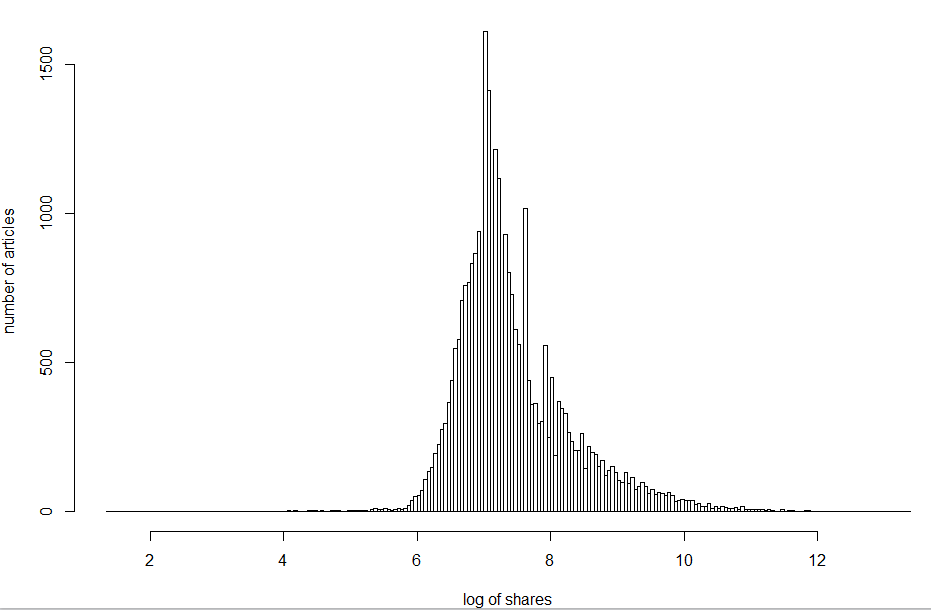
\includegraphics[width=0.7\linewidth]{logy.png}
\end{figure}

\end{frame}

%------------------------------------------------

\begin{frame}
\frametitle{Introduction}

        \centering
        \setlength\tabcolsep{2pt}  % default value: 6pt
        \tiny  %%  command to change the font size
        \scalebox{0.8}{
        \begin{tabular}{ l | l }
            \hline\hline
            Variable names & Type(\#)\\
            \hline
            \multicolumn{2}{c}{Words}\\
            \hline
            Number of words in the title & numeric(1) \\
            Number of words in the content & numeric(1) \\
            Average length of the words in the content & numeric(1) \\
            Rate of unique words in the content & numeric(1) \\
            Rate of non-stop words in the content & numeric(1) \\
            Rate of unique non-stop words in the content & numeric(1) \\
            \hline
            \multicolumn{2}{c}{Links}\\
            \hline
            Number of links & numeric(1) \\
            Number of links to other articles published by Mashable & numeric(1) \\
            Shares of referenced article links in Mashable (min, avg, max) & numeric(3) \\
            \hline
            \multicolumn{2}{c}{Digital Media}\\
            \hline
            Number of images & numeric(1) \\
            Number of videos & numeric(1) \\
            \hline
            \multicolumn{2}{c}{Time}\\
            \hline
            Days between the article publication and the dataset acquisition & numeric(1) \\
            Day of the week (from Monday to Sunday) & binary(7) \\
            The article published on the weekend & binary(1) \\
            \hline
            \multicolumn{2}{c}{Keywords}\\
            \hline
            Number of keywords in the metadata & numeric(1) \\
            Data channel (Lifestyle, Entertainment, Business, Social Media, Tech or World) & binary(6) \\
            Worst keyword shares (min, avg, max) & numeric(3) \\
            Best keyword shares (min, avg, max) & numeric(3) \\
            Average keyword shares (min, avg, max) & numeric(3) \\
            \hline
            \multicolumn{2}{c}{Natural Language Processing}\\
            \hline
            Closeness to top LDA topics from 1 to 5 & numeric(5) \\
            Text subjectivity & numeric(1) \\
            Text sentiment polarity & numeric(1) \\
            Rate of positive words in the content & numeric(1) \\
            Rate of negative words in the content & numeric(1) \\
            Rate of positive words among non-neutral tokens & numeric(1) \\
            Polarity of positive words (min, avg, max) & numeric(3) \\
            Polarity of negative words (min, avg, max) & numeric(3) \\
            Title subjectivity & numeric(1) \\
            Title polarity & numeric(1) \\
            \hline\hline
        \end{tabular}
        }
        
    
\end{frame}

%------------------------------------------------

\begin{frame}
\frametitle{Introduction}

\begin{figure}
    \centering
    \begin{subfigure}
        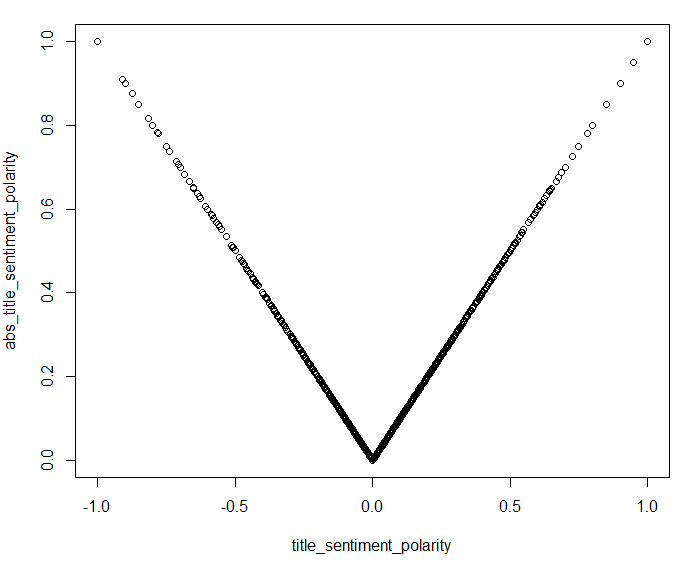
\includegraphics[width=0.3\textwidth]{data-c1.png}
    \end{subfigure}
    ~ %add desired spacing between images, e. g. ~, \quad, \qquad, \hfill etc. 
      %(or a blank line to force the subfigure onto a new line)
    \begin{subfigure}
        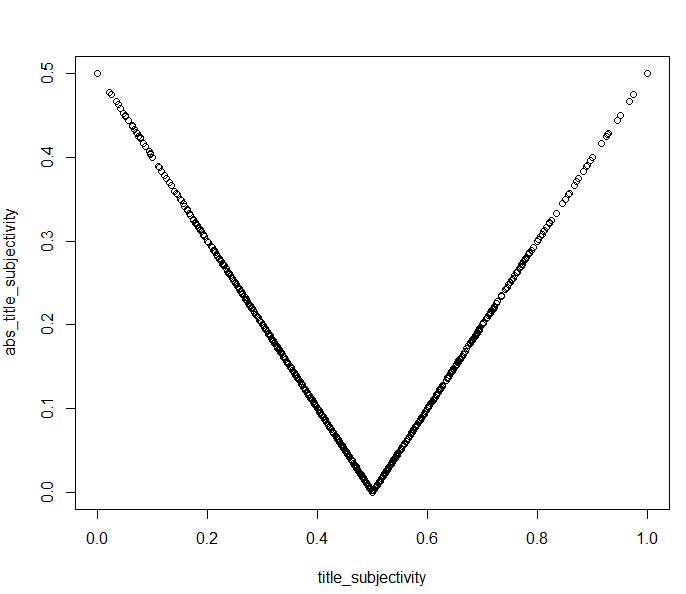
\includegraphics[width=0.3\textwidth]{data-c2.png}
    \end{subfigure}
    ~ %add desired spacing between images, e. g. ~, \quad, \qquad, \hfill etc. 
    %(or a blank line to force the subfigure onto a new line)
    \begin{subfigure}
        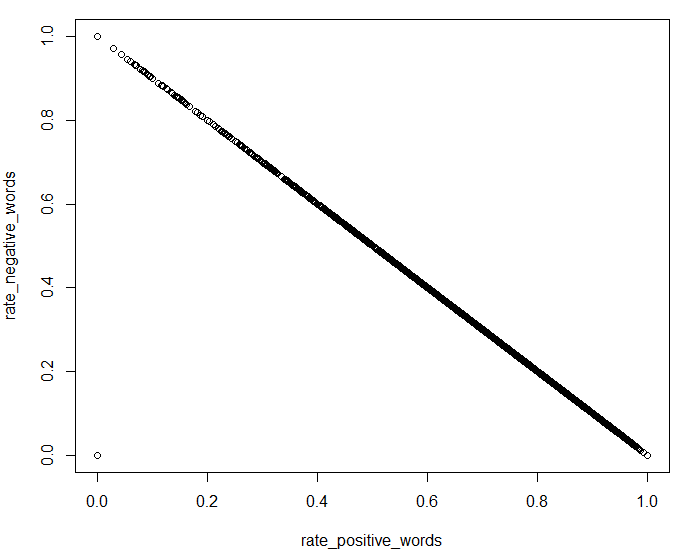
\includegraphics[width=0.3\textwidth]{data-c3.png}
    \end{subfigure}
    ~ %add desired spacing between images, e. g. ~, \quad, \qquad, \hfill etc. 
      %(or a blank line to force the subfigure onto a new line)
    \begin{subfigure}
        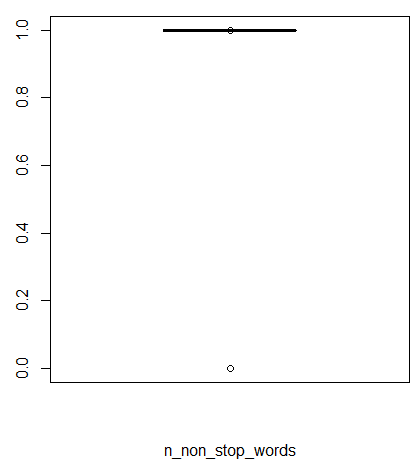
\includegraphics[width=0.3\textwidth]{data-c4.png}
    \end{subfigure}
    ~ %add desired spacing between images, e. g. ~, \quad, \qquad, \hfill etc. 
    %(or a blank line to force the subfigure onto a new line)
    \begin{subfigure}
        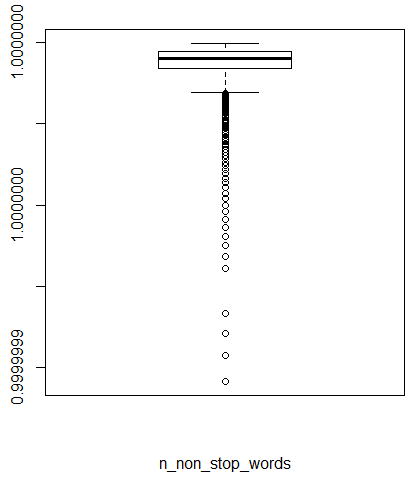
\includegraphics[width=0.3\textwidth]{data-c5.png}
    \end{subfigure}
\end{figure}

\end{frame}

%------------------------------------------------
\section{Method}
%------------------------------------------------

\subsection{Model selections} % A subsection can be created just before a set of slides with a common theme to further break down your presentation into chunks
\subsection{Regression models} % A subsection can be created just before a set of slides with a common theme to further break down your presentation into chunks
\subsection{Classification models} % A subsection can be created just before a set of slides with a common theme to further break down your presentation into chunks

%------------------------------------------------

\begin{frame}
\frametitle{Method: Model Selection}
\begin{block}{K-fold Cross-validation for parameters selecting}
Split the data randomly into K parts which are almost the same size. \\
    \begin{itemize}
      \item{Use k-th part as validation set, fit method on the rest K-1 parts}
      \item{Compute the $MSE_k$ for the observations in k-th part}
      \item{Get the CV estimation $$ CV_K = \frac{1}{K} \sum_{k=1}^{K} MSE_k$$}
    \end{itemize}

\end{block}

\begin{block}{Confusion matrix}
A confusion matrix of size n $\times$ n associated with a classifier shows the predicted and actual classification, where n is the number of different classes.
\end{block}

\end{frame}

%------------------------------------------------

\begin{frame}
\frametitle{Method: Regression Model}
\begin{block}{Linear models}
Firstly, we try to use ordinary least squares (OLS) estimates the result. If we have an input vector $X^T=(X_1,X_2,...,X_p)$, and want to predict a output Y. The linear regression model has the form $$Y=\beta_0+\sum_{j=1}^{p} X_j\beta_j + \epsilon$$
\end{block}

\begin{block}{Least Absolute Selection and Shrinkage Operator(lasso)}
OLS estimation can have low bias, but it also give a large variance. If we shrink several variable coefficients to 0, we can trade a little bit bias in order to get a smaller variance, so we may get a better prediction accuracy.
$$\min_{\beta} \sum_{i=1}^{n} (y_i-\sum_{j=1}^{p} x_{ij}\beta_{ij})^2 \text{, subject to } \sum_{j=1}^{p} \lvert \beta_j \rvert \leq t.$$
\end{block}

\begin{block}{Generalized Additive Models(GAM)}
$$Y=\alpha+\sum_{j=1}^{p} f_j(X_j)+\epsilon,$$
\end{block}

\end{frame}

%------------------------------------------------

\begin{frame}
\frametitle{Method: Regression Model}
\begin{block}{Generalized Additive Models(GAM)}
We can use some more flexible statistical methods that can show nonlinear effects. We call these methods "generalized additive models". In general, we can use a link function $g$ to relate the condition mean $\mu(X)$ of Y to an additive function: $$g[\mu(X)] = \alpha + f_1(X_1) + ... + f_p(X_p).$$
I use $g(\mu) = \mu$, the identity link, for the response data. So the additive model has the form $$Y=\alpha+\sum_{j=1}^{p} f_j(X_j)+\epsilon$$
\end{block}

\end{frame}

%------------------------------------------------

\begin{frame}
\frametitle{Method: Classification Model}
\begin{block}{Support Vector Machines(SVM)}
$$f(x) = \sum_{i=1}^{n}\alpha_i y_i K(x, x_i) + \beta_0$$
$$\text{max }L(\alpha)=\sum_{i=1}^{n} \alpha_i - \frac{1}{2}\sum_{i=1}^{n}\sum_{i'=1}^{n}\alpha_i \alpha_{i'} y_i y_{i'} K(x_i,x_{i'})$$
The kernel function:
    \begin{align}
        &\text{linear kernel}  &K(x_i,x_{i'})=<x_i,x_{i'}> \nonumber \\
        &\text{radial kernel}  &K(x_i,x_{i'})=exp(-\gamma \lVert x_i-x_{i'} \rVert^2) \nonumber
    \end{align}
\end{block}


\end{frame}

%------------------------------------------------

\begin{frame}
\frametitle{Method: Classification Model}
\begin{block}{Random Forest}
Random Forest is imporved from bagging. For growing the tree from the bootstrapped data, we select m variables at random from the p variables, instead of using all p variables to pick the best variables/split-point.
\end{block}
\begin{block}{K-Nearest Neighbors(KNN)}
K-Nearest Neighbors methods use those observations in the training set closest
in input space to x to predict $f(x)$.
$$f(x) = \text{mode}(\{ y_i \mid x_i \in N_k(x)\})$$
\end{block}


\end{frame}

%------------------------------------------------
\section{Data Analysis}
%------------------------------------------------

\subsection{Diagnostics} % A subsection can be created just before a set of slides with a common theme to further break down your presentation into chunks
\subsection{Result} % A subsection can be created just before a set of slides with a common theme to further break down your presentation into chunks

%------------------------------------------------

\begin{frame}
\frametitle{Diagnostics}
\begin{figure}
    \centering
    \begin{subfigure}
        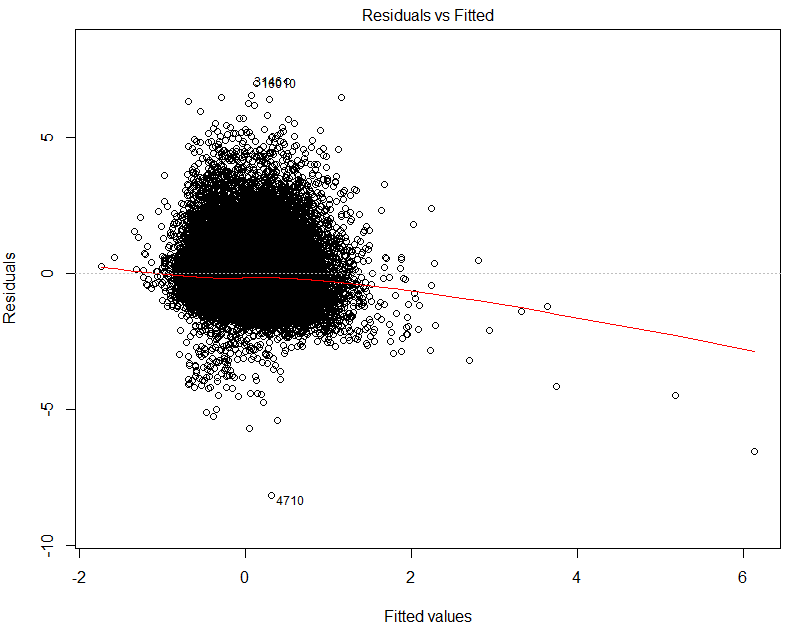
\includegraphics[width=0.4\textwidth]{linear_fvsr.png}
    \end{subfigure}
    ~ %add desired spacing between images, e. g. ~, \quad, \qquad, \hfill etc. 
      %(or a blank line to force the subfigure onto a new line)
    \begin{subfigure}
        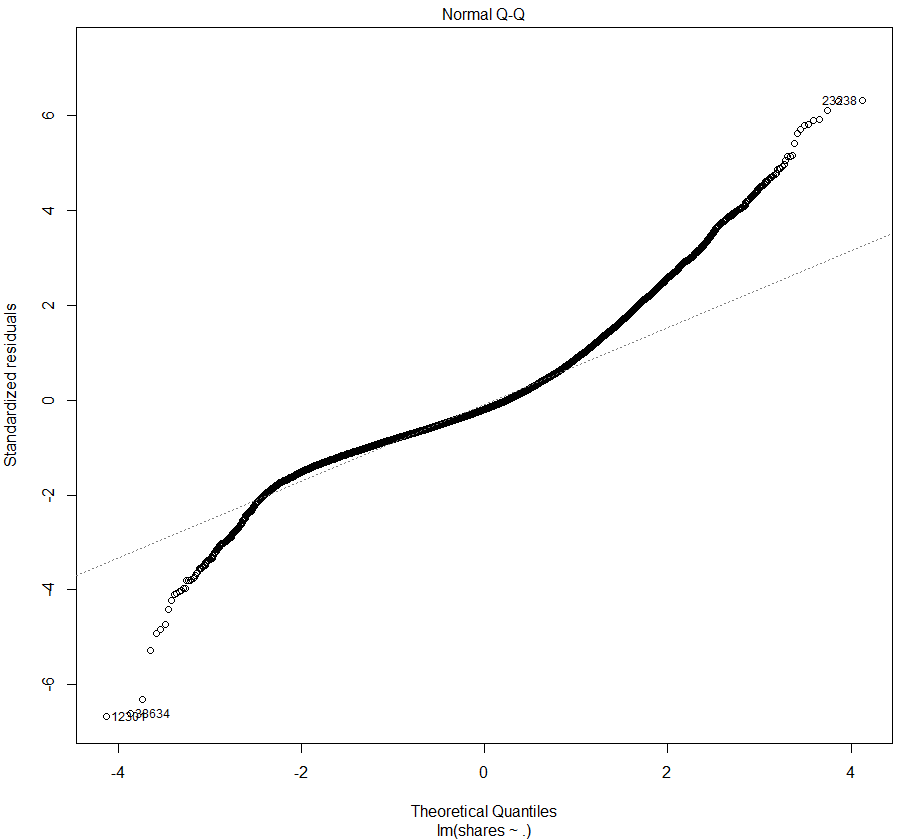
\includegraphics[width=0.4\textwidth]{linear_qq.png}
    \end{subfigure}
    ~ %add desired spacing between images, e. g. ~, \quad, \qquad, \hfill etc. 
    %(or a blank line to force the subfigure onto a new line)
    \begin{subfigure}
        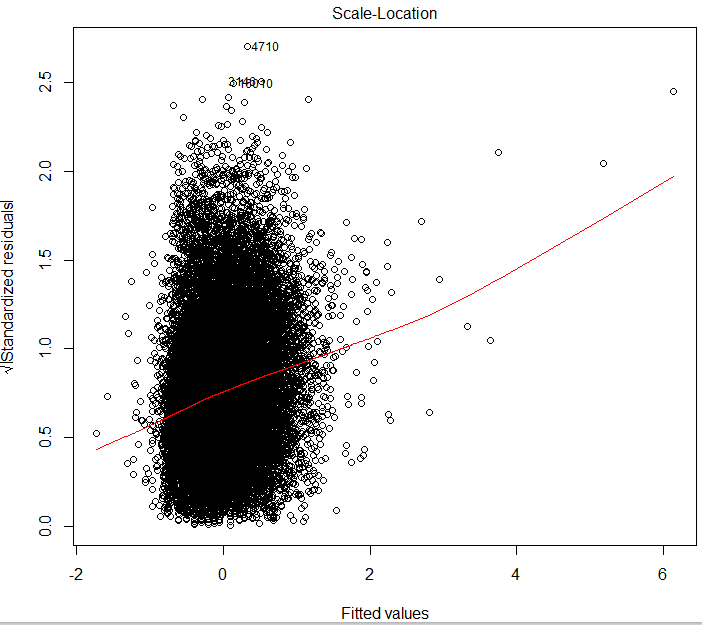
\includegraphics[width=0.4\textwidth]{linear_sl.png}
    \end{subfigure}
\end{figure}
\end{frame}

%------------------------------------------------

\begin{frame}
\frametitle{Result}
To compare each method result, I decide to separate the whole dataset into training and testing part. I use 70\% of the data to train each model, and then use the rest one to test the error.

    \begin{table}[h]
        \centering
        \caption{MSPE for Regression}
        \begin{tabular}{ l | r }
            \hline\hline
            Regression model & Testing MSPE\\
            \hline
            linear regression & 1.268389 \\
            lasso & 1.269729 \\
            GAM & 1.225438 \\
            \hline\hline
        \end{tabular}
        \label{table:1}
    \end{table}
    
\end{frame}

%------------------------------------------------

\begin{frame}
\frametitle{Result}
According to the training dataset, I decide to label the number of shares into three levels (unpopular, normal and popluar). And I use accuracy which is the percentage of correct predictions from all predictions made to describe whether the model is a good enough.

    \begin{table}[h]
        \centering
        \begin{tabular}{ l | r }
            \hline\hline
            The interval of log(shares) & Popularity\\
            \hline
            $\left[$0, 6.6746) & Unpopular \\
            $\left[$6.6746, 8.3894) & Normal \\
            $\left[$8.3894, $\infty$) & Popular \\
            \hline\hline
        \end{tabular}
    \end{table}
    
        \begin{table}[h]
        \centering
        \caption{Accuracy for classification}
        \begin{tabular}{ l | r }
            \hline\hline
            Classification model & Accuracy\\
            \hline
            SVM & 0.4429 \\
            Random forest & 0.4458085 \\
            KNN & 0.4437064 \\
            \hline\hline
        \end{tabular}
        \label{table:1}
    \end{table}
    
\end{frame}

%------------------------------------------------
\section{Conclusion}
%------------------------------------------------

\begin{frame}
\frametitle{Conclusion}
Over the regression models, the best result was achieved by Generalized Additive Model(GAM) with a testing mean squared error 1.225438 after the normalization for the log of number of shares.\\
As the classification models, the best result goes to random forest with the accuracy 0.4458085.\\
Overall, the work for this thesis gives a new perspective about the reason for influencing the popularity of online articles from a statistics view instead of content or article style. \\
In the future work, we want to use the method that the orginal thesis gives to get more data from other online articles resources to train a better model, and also try to use more method to give a better prediction.

\end{frame}

%------------------------------------------------

\begin{frame}
\Huge{\centerline{The End}}
\end{frame}

%----------------------------------------------------------------------------------------

\end{document}